\section{Results}

Figure \ref{fig:activeResult} shows the decision boundary discovered by the active learning algorithm in the 2D parameter search space for Rappahannock, SVR and San Diego regions. 
The x-axis is the parameter range of mile1 feature coefficient and y-axis represents the parameter range of the NPV feature coefficient.
The blue region (labeled as 0) represents a small number of adoptions and the red region (labeled as 1) represents a large adoptions. The notion of small and large outbreaks is defined by the $MEAN-THRESHOLD$ for each of the region. For this experiment, the settings for the three regions are given in Table \ref{tab: thresholds}. These thresholds were determined by the diagonal method described in Section \ref{sec:experiments} and Figure \ref{fig:diagDisplay}.

\begin{table}[H]
	\centering
	\caption{Thresholds for evaluating unlabelled instances.}
	\begin{tabular}{|l|l|l|}
		\hline
		{\bf Regions} & {\bf mean-threshold} & {\bf stdev-threshold} \\ 
		\hline
		Rappahannock & 1000 & 100 \\ 
		\hline
		SVR & 12000 & 3500 \\ 
		\hline
		San Diego & 120 & 12  \\ 
		\hline
	\end{tabular}
	\label{tab: thresholds}
\end{table}	
	
The red and blue points in Figure \ref{fig:activeResult} and Figure \ref{fig:alProgress} are points in the $evaluatedPoints$ set. Points are points generated around the newly found boundary point and added to this set. The classifier is trained on $evaluatedSet$. The classifier used here is Random Forest. The green points are boundary points found by the binary search algorithm described in Algorithm \ref{alg:binSearch}. Whenever a point is queried in the unlabeled space, boundary point condition is checked, followed by labeling condition. The green points are not labeled.



\begin{figure*}
\begin{subfigure}{.2\textwidth}
  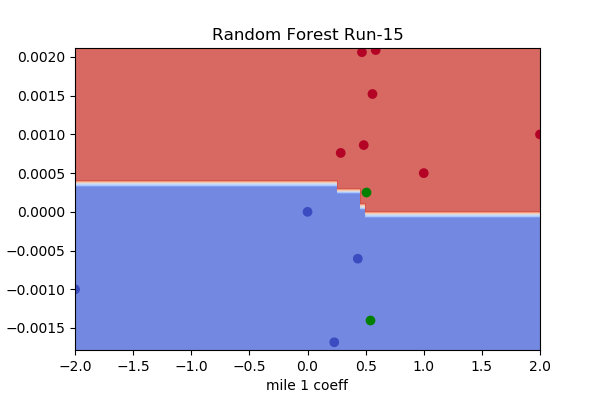
\includegraphics[width=4cm,height=3cm]{AAMAS20Template-submission/figures/RAPP-random-forest-run15.png}
  \caption{Iteration 1}
  \label{fig:diagstdev}
\end{subfigure}%
\begin{subfigure}{.2\textwidth}
  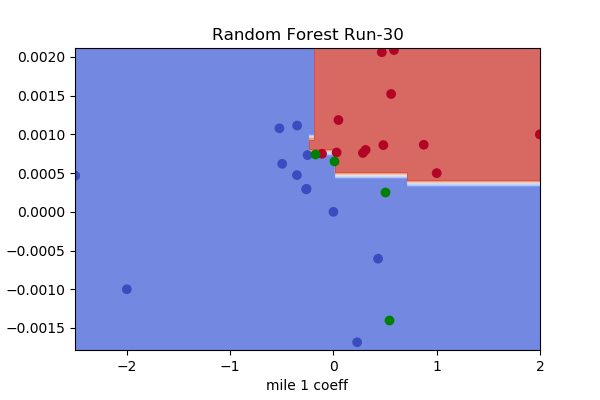
\includegraphics[width=4cm,height=3cm]{AAMAS20Template-submission/figures/RAPP-random-forest-run30.png}
  \caption{Iteration 2}
  \label{fig:}
\end{subfigure}%
\begin{subfigure}{.2\textwidth}
  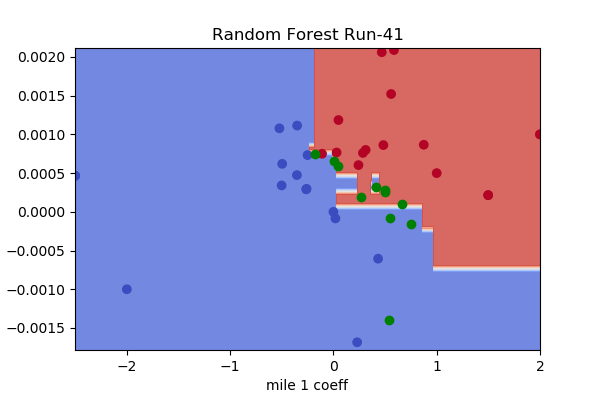
\includegraphics[width=4cm,height=3cm]{AAMAS20Template-submission/figures/RAPP-random-forest-run41.png}
  \caption{Iteration 3}
  \label{fig:}
  \end{subfigure}%
\begin{subfigure}{.2\textwidth}
  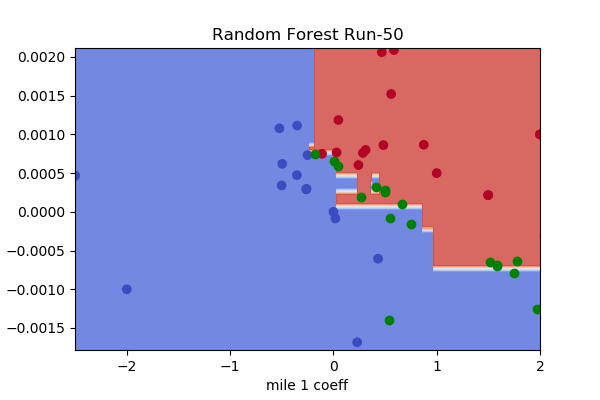
\includegraphics[width=3.7cm,height=3cm]{AAMAS20Template-submission/figures/RAPP-random-forest-run50.png}
  \caption{Iteration 4}
  \label{fig:}
\end{subfigure}
\caption{Active learning for Rappahannock : Iterations showing progress made by the active learning method to learn the decision boundary separating the bins. In our case, there are 2 bins - small outbreak (blue) and large outbreak (red). The blue and red points are used as training data for the random forest classifier.}
\label{fig:alProgress}
\end{figure*}

Figure \ref{fig:alProgress} shows how the active learning algorithm makes progress over time to learn the decision boundary with $evaluatedPoints$ on the Rappahannock region. Random forest classifier is used here. Iteration 1 shows the first time the classifier trained on the generated seed dataset. New boundary points are discovered in each iteration via binary search, followed by training the classifier on the incremental set of $evaluatedPoints$. Finally, we can observe the sensitivity of mile 1 and NPV feature coefficients with respect to the simulation output variable $y$.

% DO NOT DELETE THIS
%RAPP
%Bin0 = label 0 = small outbreak = 11960953
%Bin1 = label 1 = large outbreak = 5052827
%Rappahannock Probability of bin0=label0=small outbreak=blue :: 0.703015614401973
%Rappahannock Probability of bin1=label1=large outbreak=red :: 0.29698438559802703

%SanDiego
%Bin0 = label 0 = small outbreak = 4794233
%Bin1 = label 1 = large outbreak = 7037217
%SanDiego Probability of bin0=label0=small outbreak=blue :: 0.40521094202316704
%SanDiego Probability of bin1=label1=large outbreak=red :: 0.5947890579768329


Figure \ref{fig:characteristicDistri} shows the characteristic distributions of 2 bins for our ABMs. 
Bin 1 (blue color) represents small outbreak probability and bin 2 (red color) represents large outbreak probability. {\color{magenta}DESCRIBE results once in }

%This distance is also known as the earth mover’s distance, since it can be seen as the minimum amount of “work” required to transform  into , where “work” is measured as the amount of distribution weight that must be moved, multiplied by the distance it has to be moved.
In order to calculate the distance between these distributions, we will use Equation \ref{eq:charDist}, where $D$ is chosen to be earth mover’s distance. Refer Table \ref{tab: characterDistancesABM} to see what is the minimum amount of work required to transform from one probability distribution to the other.

\begin{table}[H]
	\centering
	\caption{Characteristic distance: Minimum amount of work required to transform from distribution $u$ to $v$ given by earth mover's distance.}
	\begin{tabular}{|l|l|l|}
		\hline
		{\bf $u$} & {\bf $v$} & {\bf EMD} \\ 
		\hline
		Rappahannock & San Diego & 100 \\ 
		\hline
		Rappahannock & SVR & 3500 \\ 
		\hline
		San Diego & SVR & 12  \\ 
		\hline
		San Diego & Rappahannock & 12  \\ 
		\hline
		SVR & Rappahannock & 12  \\ 
		\hline
		SVR & San Diego & 12  \\ 
		\hline
	\end{tabular}
	\label{tab: characterDistancesABM}
\end{table}	





We also look at disagreement between the two ABMs. Equation \ref{eq:disagreement}, defines disagreement between two ABMs as a choosing a probability setting of parameters that results in a difference in the simulation output $y$ of the two models. Figure  shows -------------------------------------------- the disagreement between the pairs of models. {\color{magenta}DESCRIBE }



\begin{figure*}
\begin{subfigure}{.3\textwidth}
  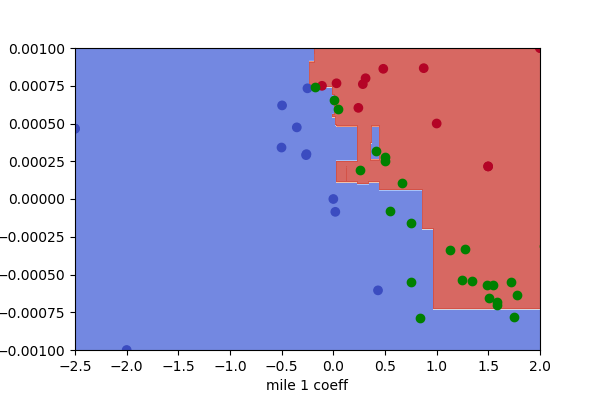
\includegraphics[width=5.5cm,height=4cm]{AAMAS20Template-submission/figures/rapp-book17-final-RF.png}
  \caption{Rappahannock}
  \label{fig:diagstdev}
\end{subfigure}%
\begin{subfigure}{.3\textwidth}
  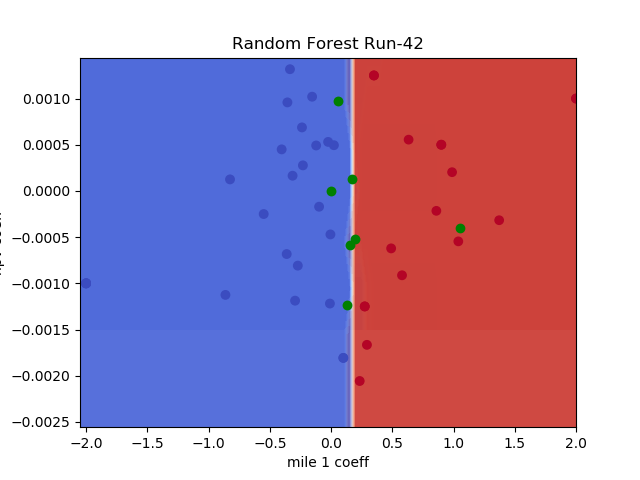
\includegraphics[width=5.5cm,height=4cm]{AAMAS20Template-submission/figures/svrbook6-random-forest-run42.png}
  \caption{SVR (placeholder)}
  \label{fig:}
\end{subfigure}%
\begin{subfigure}{.3\textwidth}
  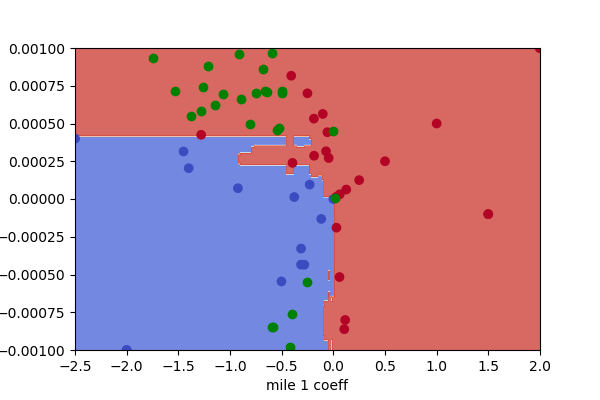
\includegraphics[width=5.5cm,height=4cm]{AAMAS20Template-submission/figures/sandia-book9-RF.png}
  \caption{San Diego}
  \label{fig:}
\end{subfigure}
\caption{Decision boundary discovered by the active learning algorithm in the 2D parameter search space for Rappahannock, SVR and San Diego regions. The blue region (labeled as 0) represents a small number of adoptions and the red region (labeled as 1) represents a large adoptions. The x-axis is the range of mile1 feature coefficient and y-axis represents range of the NPV feature coefficient.}
\label{fig:activeResult}
\end{figure*}


\begin{figure}
    \centering
    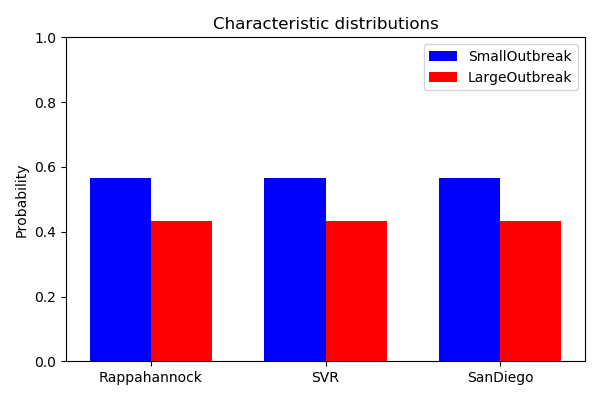
\includegraphics[height=6cm,width=8cm]{AAMAS20Template-submission/figures/CharacteristicDistributions.png}
    \caption{<PLACEHOLDER> Characteristic Distributions of ABMs for Rappahannock, SVR and San Diego regions.}
    \label{fig:characteristicDistri}
\end{figure}